\documentclass{article} % For LaTeX2e
\usepackage{nips13submit_e,times}
\usepackage{hyperref}
\usepackage{url}
\usepackage{amsmath}
\usepackage{graphicx}

\title{Learning words through recursive pragmatic reasoning about other agents}

\author{
Nathaniel Smith\thanks{...} \\
School of Informatics\\
University of Edinburgh\\
Edinburgh, Scotland, UK\\
\texttt{nathaniel.smith@ed.ac.uk} \\
\AND
Noah D. Goodman \\
Department of Psychology\\
Stanford University \\
Stanford, CA, USA \\
\texttt{ngoodman@stanford.edu} \\
\And
Michael C. Frank \\
Department of Psychology \\
Stanford University \\
Stanford, CA, USA \\
\texttt{mcfrank@stanford.edu}}

\newcommand{\fix}{\marginpar{FIX}}
\newcommand{\new}{\marginpar{NEW}}

\newcommand{\word}{\text{word}}
\newcommand{\obj}{\text{object}}

% \nipsfinalcopy % Uncomment for camera-ready version

\begin{document}

\maketitle

\begin{abstract}
  Adult language users are remarkably good at making inferences about speakers' intentions in context, and children learning their native language also display substantial pragmatic skill in acquiring the meanings of unknown words. While pragmatic inference and word learning have both been characterized in probabilistic terms, no current models make appropriate inferences about the meanings of words in pragmatically-rich inferential contexts. We describe a model in which language learners assume that they jointly approximate a shared, external lexicon and reason recursively about the goals of others in using this lexicon. This model captures phenomena in word learning and pragmatic inference; it additionally leads to insights about the emergence of communicative systems in conversation and the mechanisms by which pragmatic inferences become incorporated into word meanings.
\end{abstract}

\section{Introduction}

Natural language is a powerful tool for conveying meaning in context. Our utterances are pervasively underspecified. Consider ``it's raining,'' ``I ate some of the cookies,'' or ``can you close the window?'' In each, a listener must go beyond the literal meaning of the words to fill in contextual details (``it's raining here and now''), infer that a stronger alternative is not true (``I ate some but not all of the cookies''), or more generally infer the speaker's communicative goal (``I want you to close the window right now because I'm cold.'').

Following this intuition, theories of pragmatic communication frame the process of language comprehension as inference about the generating goal of an utterance given a rational speaker \cite{grice1975,dale1995,frank2012}. For example, a listener might reason, ``if she had wanted me to think `all' of the cookies, she would have said `all'---but she didn't. Hence `all' must not be true and she must have eaten some {\it but not all} of the cookies.'' This kind of counterfactual reasoning has a recursive character to it: listener models speaker (who may in turn be modeling a listener).

Even before they are proficient language users, children learn the meanings of words from their pattern of use in context. For example, in demonstrations of the ``disambiguation effect,'' a novel word (e.g. ``dax'') is used in a context containing both a novel and a familiar object. From quite young, children tend to make the inference that ``dax'' refers to the novel object \cite{markman1988}. In another demonstration, even young toddlers can extract mappings between words and objects from a pattern of individually-ambiguous co-occurrences between pairs of words and pairs of objects \cite{smith2008}. Taking inspiration from children's learning prowess, recent work in the field of grounded language learning has explored the possibility that even relatively complex word meanings can be inferred from corpus data (e.g. \cite{zettlemoyer2005,chen2008,frank2009,kwiatkowski2010,johnson2012}).

Recursive pragmatic inferences such as those described above could be an important part of language learning.\footnote{Very young children make inferences that are often labeled as ``pragmatic'' in that they involve reasoning about context \cite{clark1988,baldwin1993}, though they also show weaknesses in specific inferences (e.g. strengthening ``some'' to ``some but not all'' \cite{papafragou2003}). Here we remain agnostic about the age at which children are able to make such inferences robustly, as it may vary depending on the linguistic materials being used in the inference \cite{barner2011}.} For example, the disambiguation inference described above can emerge from such reasoning (``why would the speaker have said ``dax'' if there was a word for the known object that she knew I would know'') \cite{clark1988}. In addition, there are a variety of intriguing cases in which listeners seem to create situation- and task-specific ways of referring to particular objects. For example, when asked to refer to idiosyncratic geometric shapes, over the course of an experimental session, participants create conventionalized descriptions that allow them to perform accurately even though they do not begin with a shared label \cite{krauss1964,clark1986}. Yet models of grounded language learning have failed to take pragmatic factors into account.

The goal of our current work is to investigate the possibilities for integrating models of recursive pragmatic reasoning with models of language learning, with the hope of capturing phenomena in both domains. We begin by describing previous models in each domain as well as proposals for bringing the two together. We next simulate findings from the domains of pragmatic inference, word learning, and their intersection (summarized in Table \ref{tab:results}). We end by discussing the implications of our results for work on language change.

\section{Models}

Consider a simple communicative game: two participants each,
separately, view identical arrays of objects. On the
\textit{Speaker's} screen, one object is highlighted; their goal is to
get the \textit{Listener} to click on this item. To do this, they have
available a fixed, finite set of words; they must pick one. The
Listener then receives this word, and attempts to guess which object
the Speaker meant by it.

This suggest a simple probabilistic model. Given any particular
decision procedure used by the Speaker $S$, the optimal way for the
Listener $L$ to judge the probability of each object is to invert this
decision procedure using Bayes' rule, taking into account the prior
likelihood of each object:
\begin{align*}
P_L(\obj | \word) &\propto P_S(\word | \obj) P_{\text{prior}}(\obj |
\text{context})
\end{align*}
$S$, meanwhile, being herself a rational Bayesian agent, chooses her
word so as to soft-maximize a utility function $U(\word | \obj)$. She
gains utility if $L$ is likely to understand her; she loses utility if
the word is particularly costly to say (e.g., it may be long).
\begin{align*}
P_S(\word | \obj) &\propto \exp \lambda U(\word | \obj) \\
U(\word | \obj) &= \log P_L(\obj | \word) - \text{cost}(\word)
\end{align*}
The degree to which she optimizes this utility is controlled by the
softmax parameter $\lambda$. If $\lambda = 1$ and all words cost the
same, then her probability of producing a word will be proportional to
the likelihood that it will cause $L$ to reach the correct
interpretation; as $\lambda$ increases, she becomes more likely to
choose the word which maximizes this likelihood. (We somewhat
arbitrarily set $\lambda = 3$ throughout.)

This model as stated is optimal by various criteria, but suffers from
a fatal flaw: $S$'s decision procedure depends on $L$'s interpretive
procedure, and vice-versa. This means that it can only be implemented
as stated for a very spei

And indeed, in similar games, humans seem to reason only a few levels
deep (XX cite p-beauty contests), and

Basic idea of iterated pragmatic reasoning models. $S_i$ defines a causal model for utterances described by a simple Bayes net. $L_{i+1}$ does standard rational inference over this network. But the likelihood function in $S_i$'s model is very complicated, and includes equations derived from considering how a hypothetical $L_{i-1}$ would interpret utterances if they were doing rational inference about another hypothetical causal agent $S_{i-2}$.

To simplify matters we envision a simple world that has $k$ words and $l$ objects. The \textit{lexicon} defines the literal meaning of each word, ...

extensional as marginalization over intensional

\begin{align*}
P_{L_0}(\obj | \word) &= \text{lexicon}(\word, \obj) P_{\text{prior}}(\obj | \text{context}). \\
P_{S_i}(\word | \obj) &\propto \exp\Big(\lambda \big(\log P_{L_{i - 1}}(\obj | \word) - \text{cost}(\word)\big)\Big) \\
P_{L_i}(\obj | \word) &\propto P_{S_{i-1}}(\word | \obj) P_{\text{prior}}(\obj | \text{context})
\end{align*}

\subsection{Naive literal learner model}



To see how
Make $L_0$ uncertain about values in $\text{lexicon}(\word, \obj)$, impose a prior, and then

Needs feedback

can't switch roles from speaker to listener

knocks out the lexical uncertainty/horn implicature results (because you can only have uncertainty at one level)

something wrong about taking evidence from the pragmatic speaker and using it to train the literal listener

\subsection{``Social anxiety'' model}

\section{Experiments 1: Empirical coverage}

In this section, we describe the coverage of our pragmatic learning model on phenomena previously investigated with the pragmatics and word learning components of the model. To summarize these simulations: the pragmatic learning model reproduces previous findings and provides some new insights into the ``disambiguation'' phenomenon described above. 

\begin{table}[t]
\label{tab:results}
\begin{center}
\begin{tabular}{lccccc}
\hline \\
Phenomenon & Ref. & WL & PI & Lifted PI  & PIL \\
\hline
Scalar implicature & \cite{grice1975} &  & x &x & x\\
Horn implicature & \cite{horn1984} & &  & x& x\\
Cross-situational learning & \cite{smith2008} & x& & & x \\
Disambiguation & \cite{markman1988} &x  & & & x \\
Communicative equilibria & \cite{galantucci2005} & & & & x \\
\hline
\end{tabular}
\end{center}
\caption{Empirical results and references. WL refers to the word learning model of \cite{frank2009}; PI refers to the pragmatic inference model of \cite{frank2012}; Lifted PI refers to the pragmatic inference model of \cite{bergen2012}, and PIL refers to the pragmatic inference and learning model described here.  }

\end{table}


\subsection{Scalar implicature}

Many sets of words in natural language form scales in which each term refers to successively stronger restrictions on the situations compatible with the term. ``Some'' and ``all'' form a scale of this type. While ``I ate some of the cookies'' is compatible with the followup ``in fact, I ate {\it all} of the cookies,'' the reverse is not true. ``Might'' and ``must'' are another example, as are ``OK,'' ``good,'' and ``excellent.'' All of these scales allow for {\it scalar implicatures} \cite{grice1975}: if a speaker uses a weaker term, a listener is licensed to infer that the stronger term was not true in this situation. So although ``I ate some of the cookies'' could in principle be compatible with eating all of them, the listener is lead to believe that ``some but not all'' is the likely state of affairs. 

The recursive pragmatic reasoning portions of our model capture set of findings on scalar implicature effectively. Consider a representation of scalar implicature as a matrix 
$\left[
    \begin{array}{cc}
      1 & 1 \\
      0 & 1
    \end{array} 
  \right]$,
where rows show the terms ``some'' and ``all'' and columns indicate worlds where {\sc some} and {\sc all} are true, respectively, capturing the regularity that ``some'' can be said of situations where {\sc all} is actually the case. Assuming uniform costs for the two words and uniform priors, each recursion of listener modeling speaker reduces the probability that ``some'' will be used to refer to {\sc all}. Using the fixed parameters employed in our other simulations results in speaker use probabilities of 
$\left[
    \begin{array}{cc}
      1.00 & 0.00 \\
      0.00 & 1.00
    \end{array} 
  \right]$
and listener interpretation probabilities of 
$\left[
    \begin{array}{cc}
      .86 & .14 \\
      .03 & .97
    \end{array} 
  \right]$.

% Simulation parameters:
%   prior on meaning of "some": dirichlet(10, 10)
%   prior on meaning of "all": dirichlet(1, 10)
%
% How speaker refers to "some" and "all" objects:
% array([[  9.99951162e-01,   2.87541198e-03],
%        [  4.88378335e-05,   9.97124588e-01]])
%
% How listener interprets "some" and "all" words:
% array([[ 0.86214895,  0.13785105],
%        [ 0.03151434,  0.96848566]])

\subsection{Horn implicature}

Horn implicatures are inferences where the critical factor is not the extension of the words in context (as in scalar implicatures), but instead the relative cost of two expressions. In Horn's example, ``Lee got the car to stop'' implies that Lee used an unusual method (e.g. not the brakes) because, had he used the brakes, the speaker would have chosen the simpler and shorter (less costly) expression, ``Lee stopped the car.'' In other words, the costly expression is assumed to be associated with the unusual outcome.

Such an implicature again arises naturally from our model. We create a situation in which expressions have differential costs (e.g. $[.5 1.0]$) and referents have differential probabilities (e.g. $[.8 .2]$). Speakers in such a situation choose simple words to refer to common referents, e.g. 
$\left[
    \begin{array}{cc}
      .88 & .54 \\
      .12 & .46
    \end{array} 
  \right]$.\footnote{Rows indicate words and columns indicate referents. For speakers, columns are normalized to indicate a distribution over words to be produced given referents, and for listeners rows are normalized to indicate a distribution on referents given words heard.} Similarly, listeners interpret ``cheap'' and ``expensive'' words to refer to common and rare objects respectively:
$\left[
    \begin{array}{cc}
      .77 & .23 \\
      .65 & .35
    \end{array} 
  \right]$.


% Simulation parameters:
%   word costs: 0.5, 1.0
%   object prior: 0.8, 0.2
%
% How speaker refers to "common" and "rare" objects:
% array([[ 0.88491473,  0.53858973],
%        [ 0.11508527,  0.46141027]])
%
% How listener interprets "cheap" and "expensive" words:
% array([[ 0.77458316,  0.22541684],
%        [ 0.64702551,  0.35297449]])

\subsection{Statistical cross-situational word learning}

A recent line of work in language acquisition has 
% \begin{figure}[t]
%   \centering
%   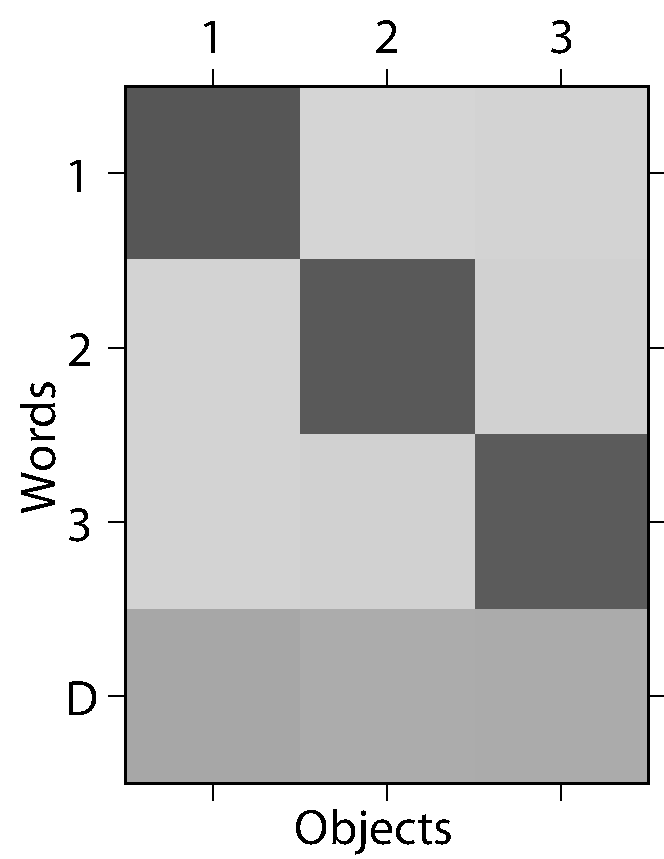
\includegraphics[width=0.20\textwidth]{figures/cross-sit.pdf}
%   \caption{Cross-situational simulation}
%   \label{fig:cross-sit}
% \end{figure}

\subsection{Disambiguation using known words}

% Novel word means: Familiar object: 25.5%. Novel object: 74.5%.
% To anti-sparse listener, novel word means: Familiar object: 21.4%. Novel object: 78.6%.
% To sparse listener, novel word means: Familiar object: 30.5%. Novel object: 69.5%.

\begin{figure}[t]
  \centering
  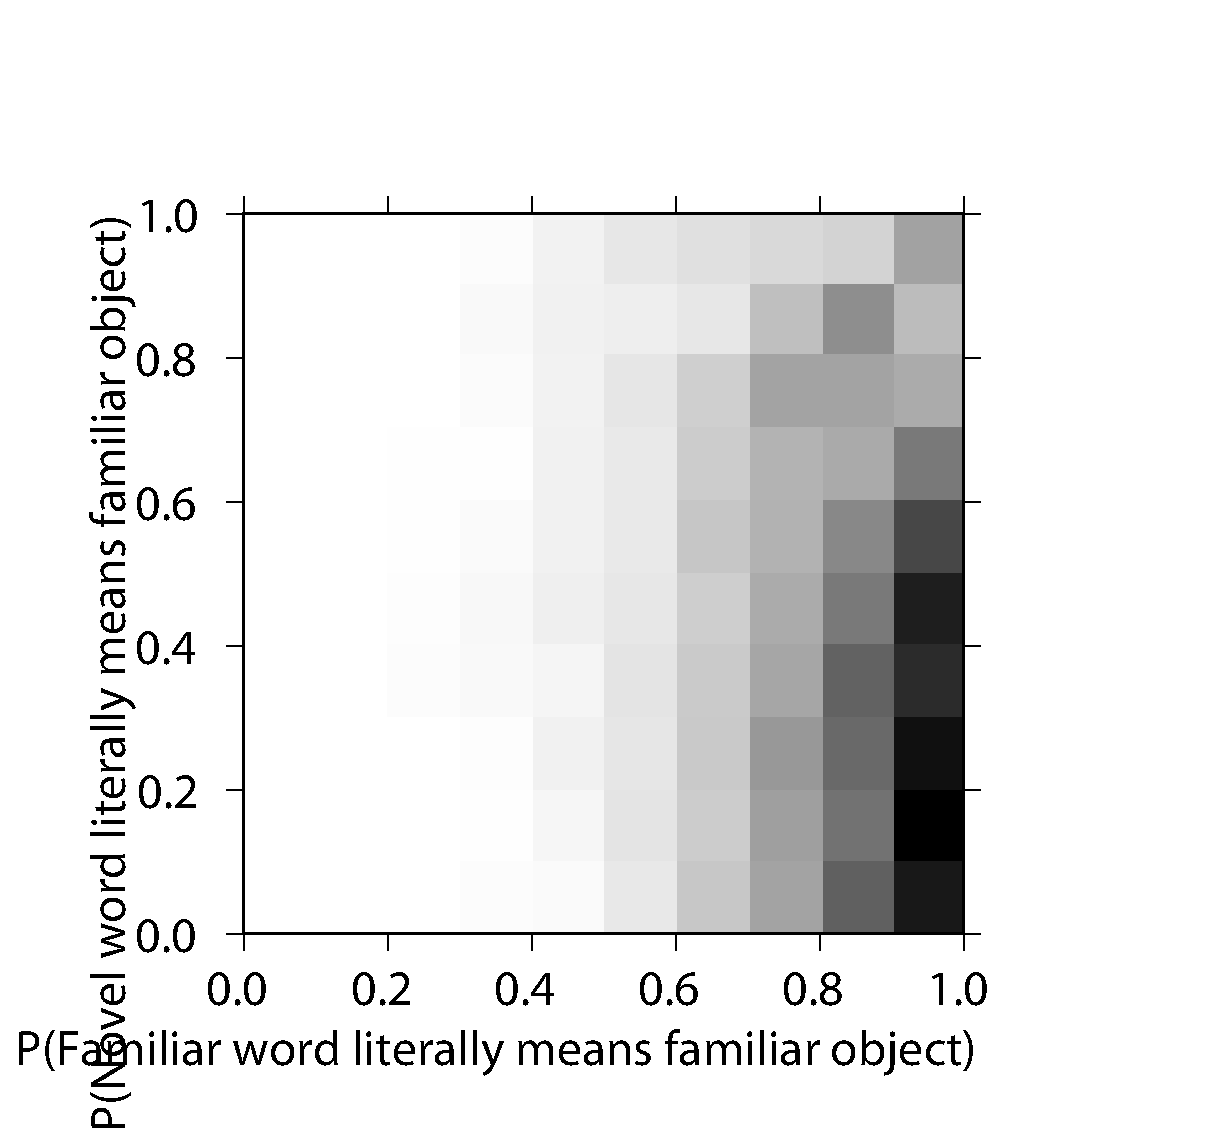
\includegraphics[width=0.20\textwidth]{figures/ME-1dax.pdf}
  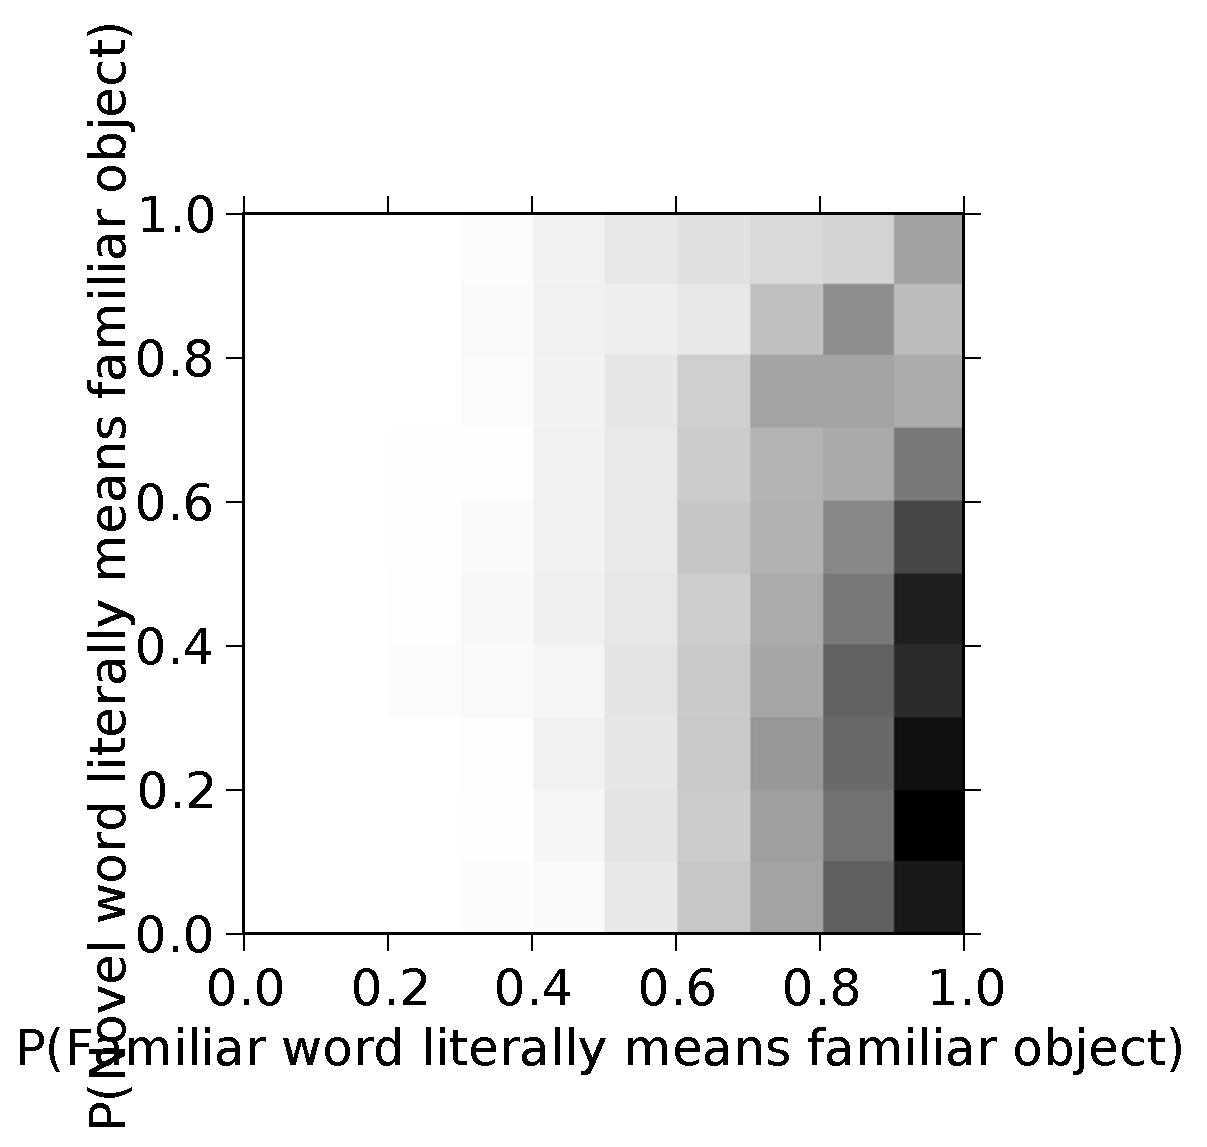
\includegraphics[width=0.20\textwidth]{figures/ME-flat-10dog-10dax.pdf}
  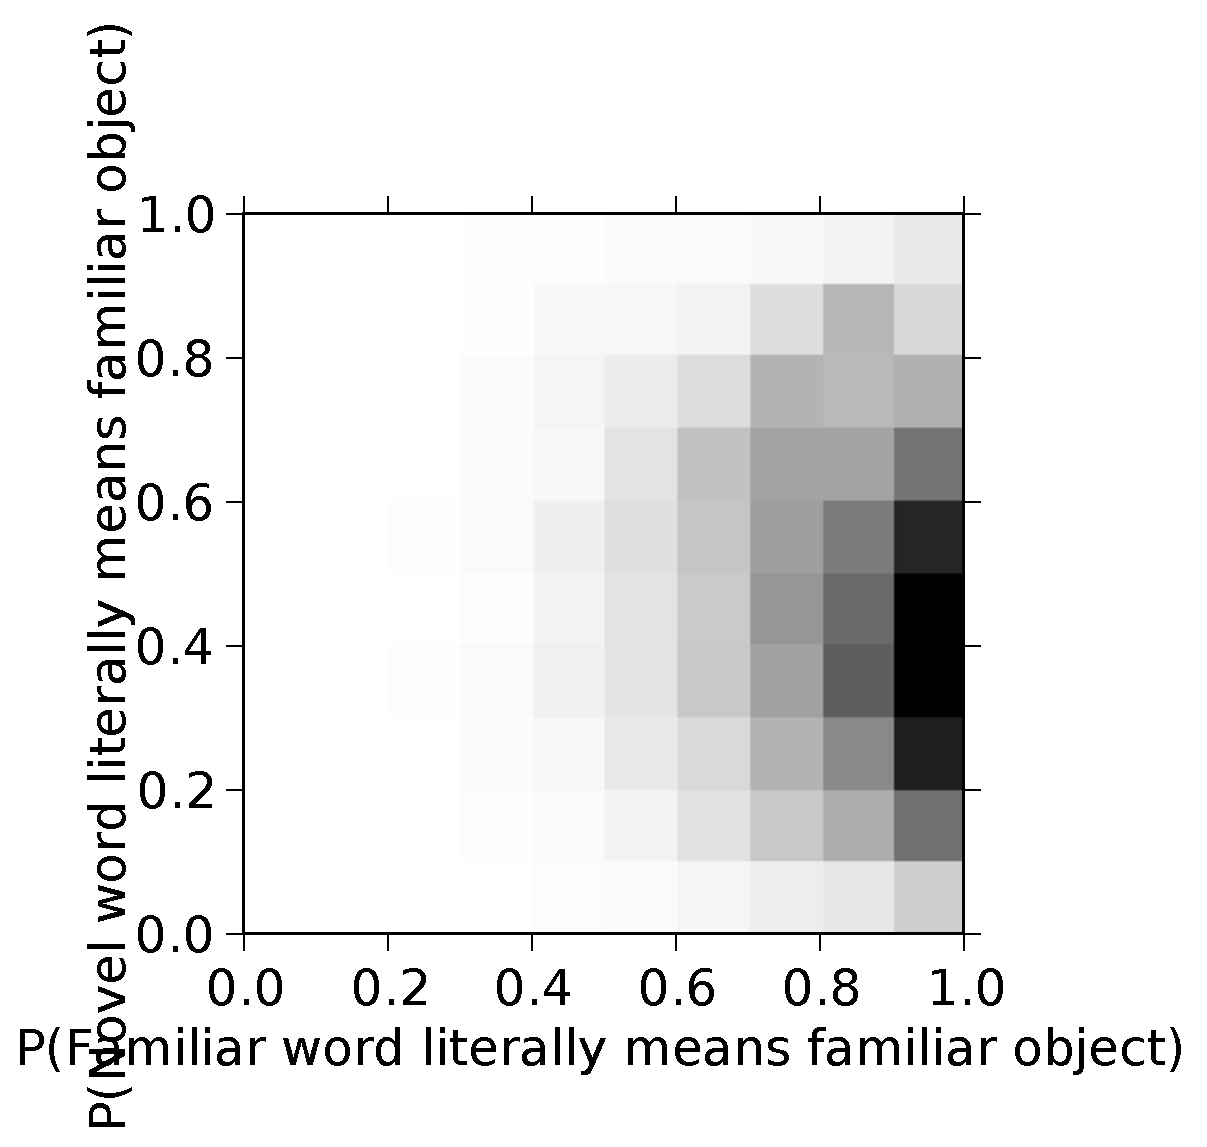
\includegraphics[width=0.20\textwidth]{figures/ME-antisparse-10dog-10dax.pdf}
  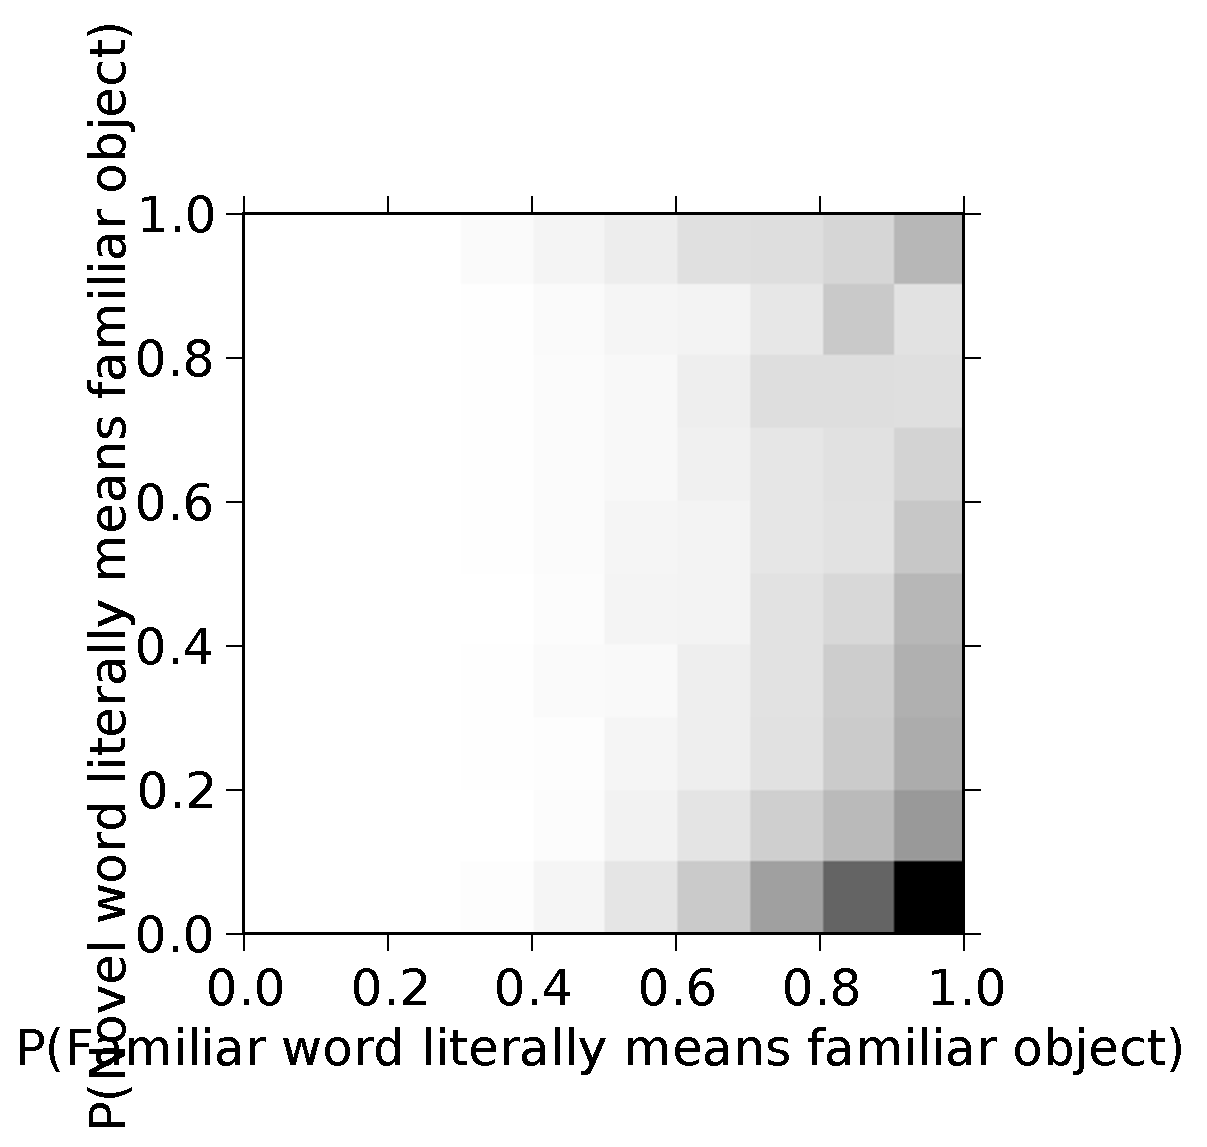
\includegraphics[width=0.20\textwidth]{figures/ME-sparse-10dog-10dax.pdf}
  \caption{Mutual exclusivity simulation}
  \label{fig:mutual-exclusivity}
\end{figure}

\section{Experiments 2: Lexical learning in pragmatic contexts}

\subsection{Emergence of communicative equilibria}

\begin{figure}[t]
\centering
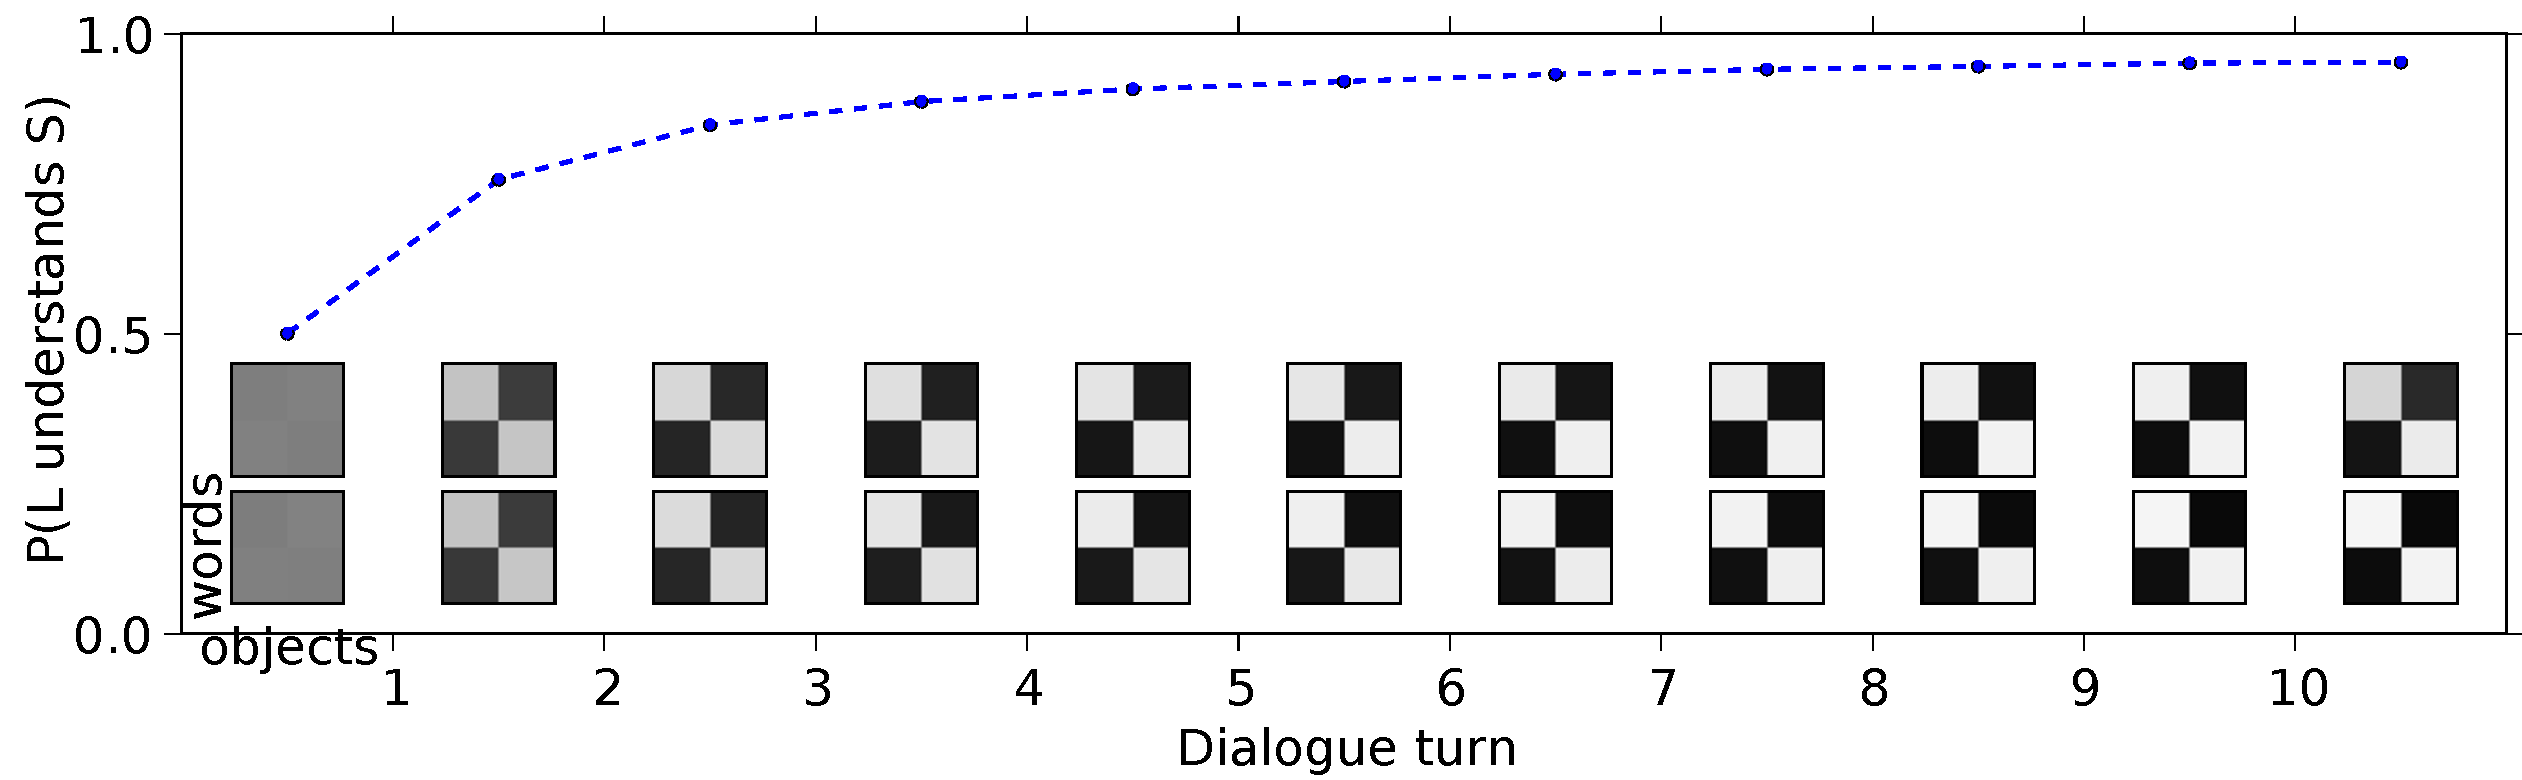
\includegraphics[width=0.48\textwidth]{figures/emergence2x2-1.pdf}
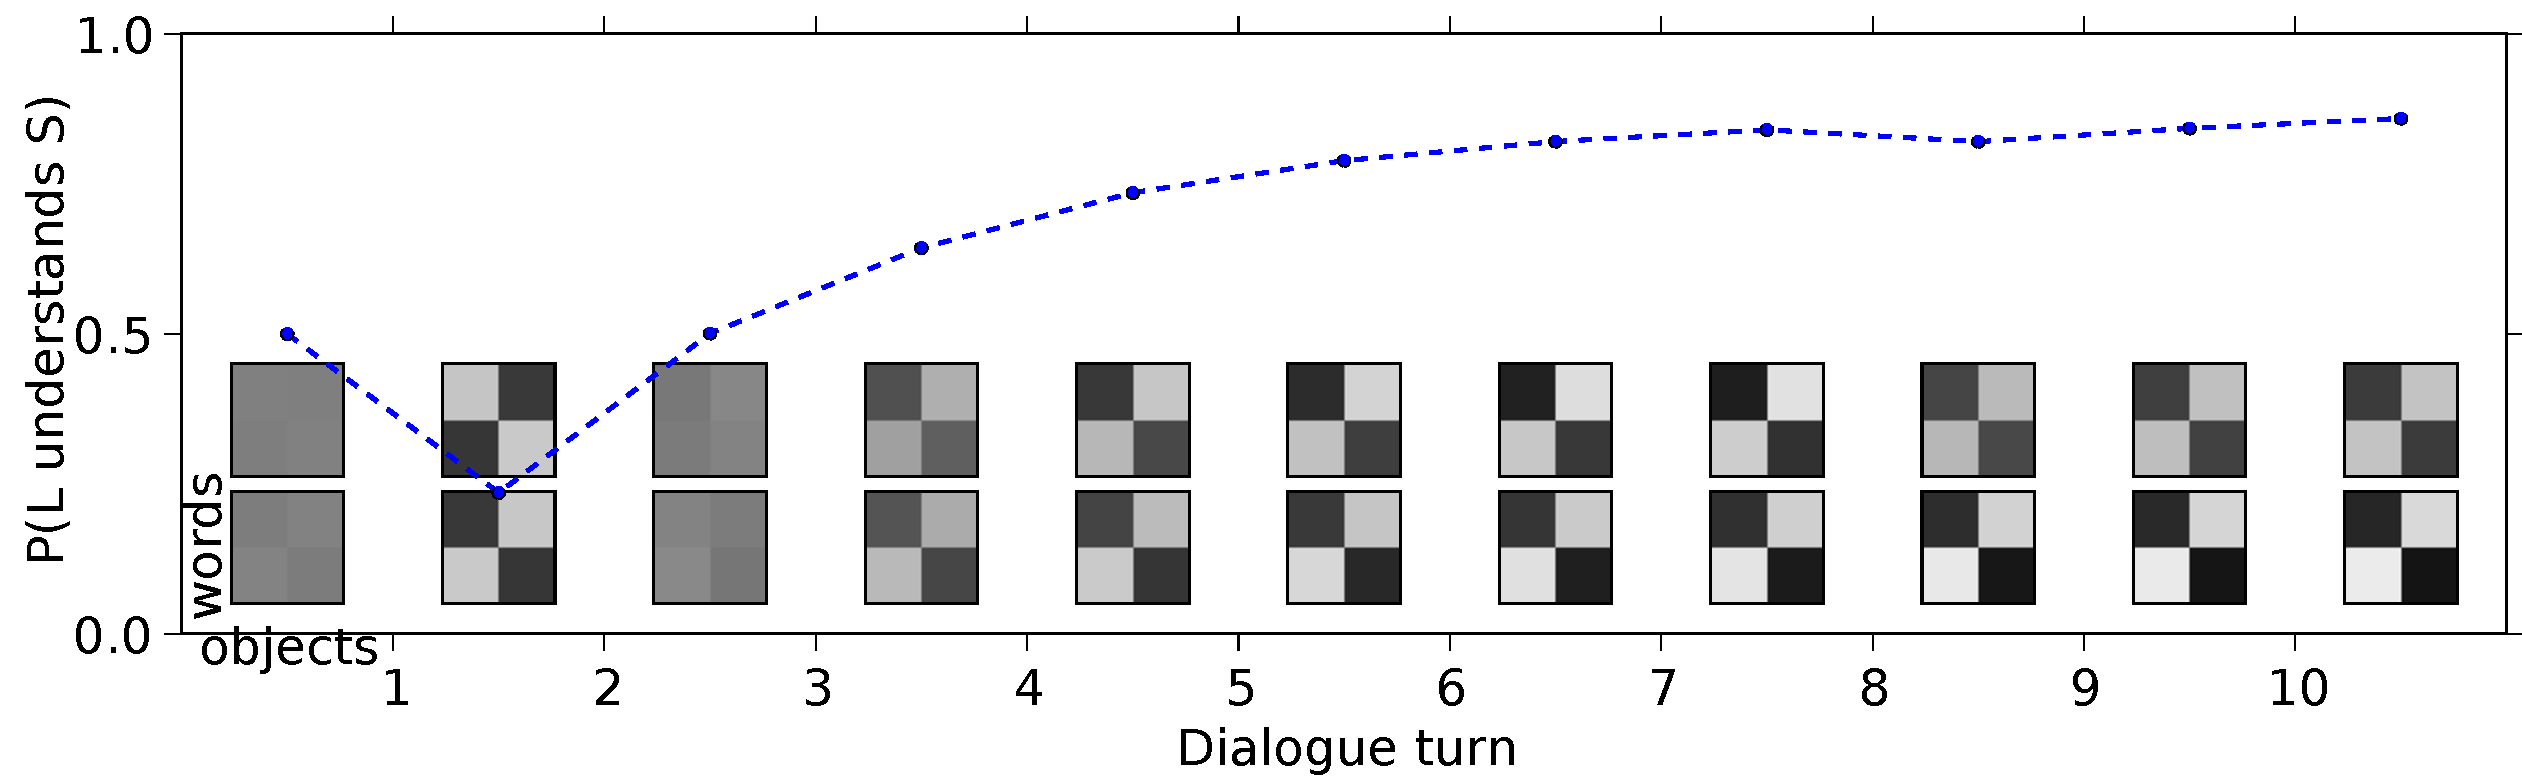
\includegraphics[width=0.48\textwidth]{figures/emergence2x2-3.pdf} \\
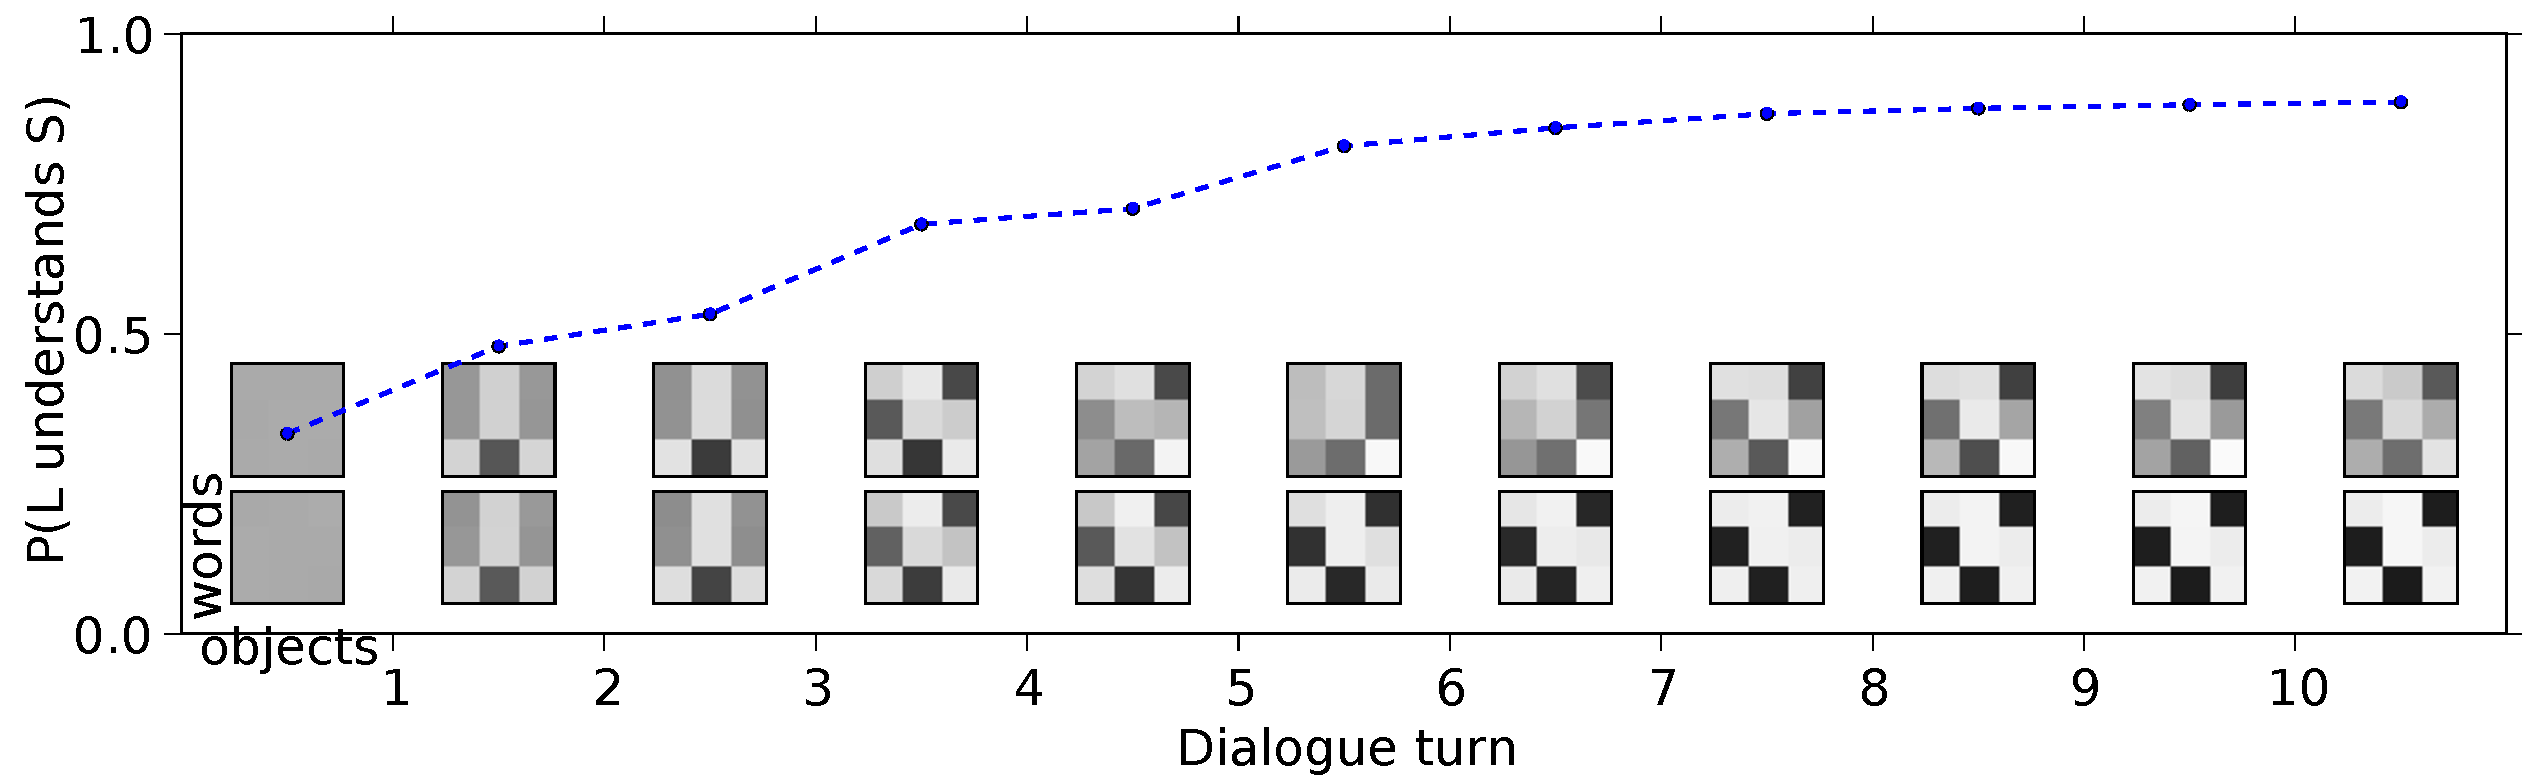
\includegraphics[width=0.48\textwidth]{figures/emergence3x3-0.pdf}
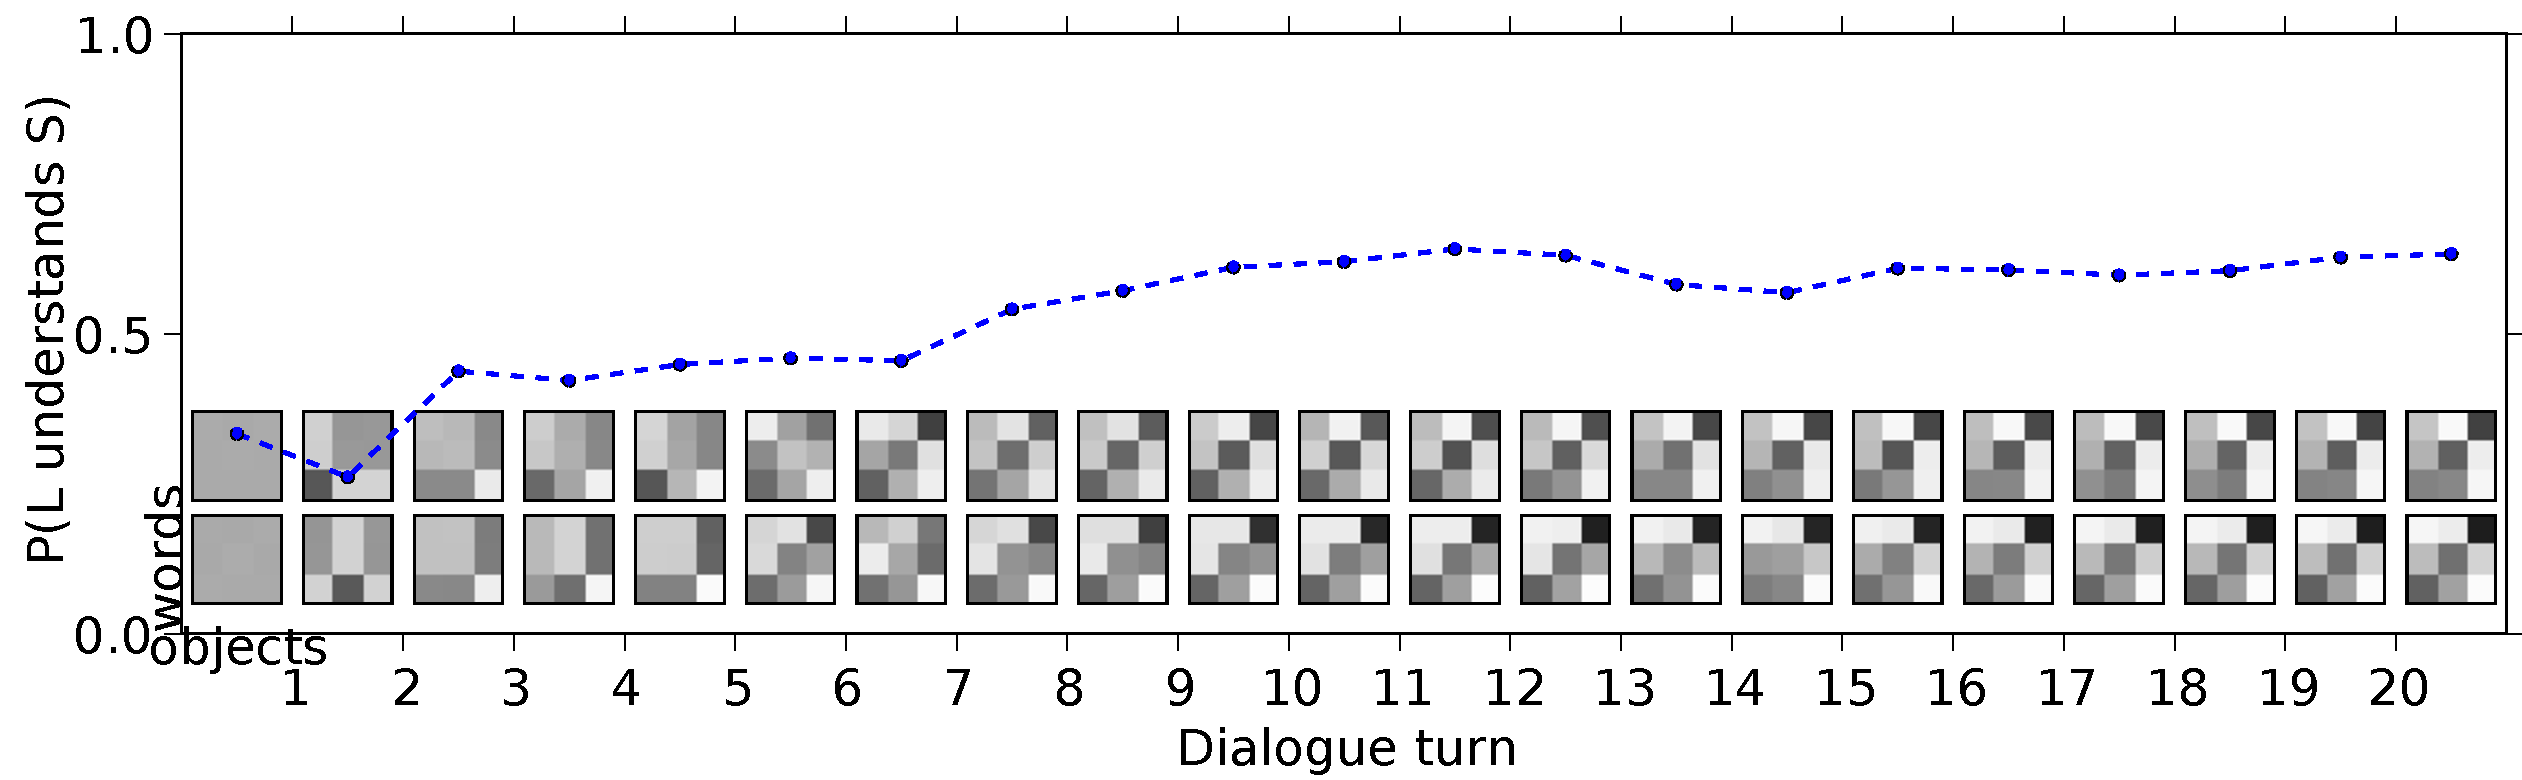
\includegraphics[width=0.48\textwidth]{figures/emergence3x3-1.pdf} \\
\caption{\label{fig:emergence} Simulations....}
\end{figure}

\subsection{Lexicalization of Horn implicatures}

\begin{figure}[t]
\centering
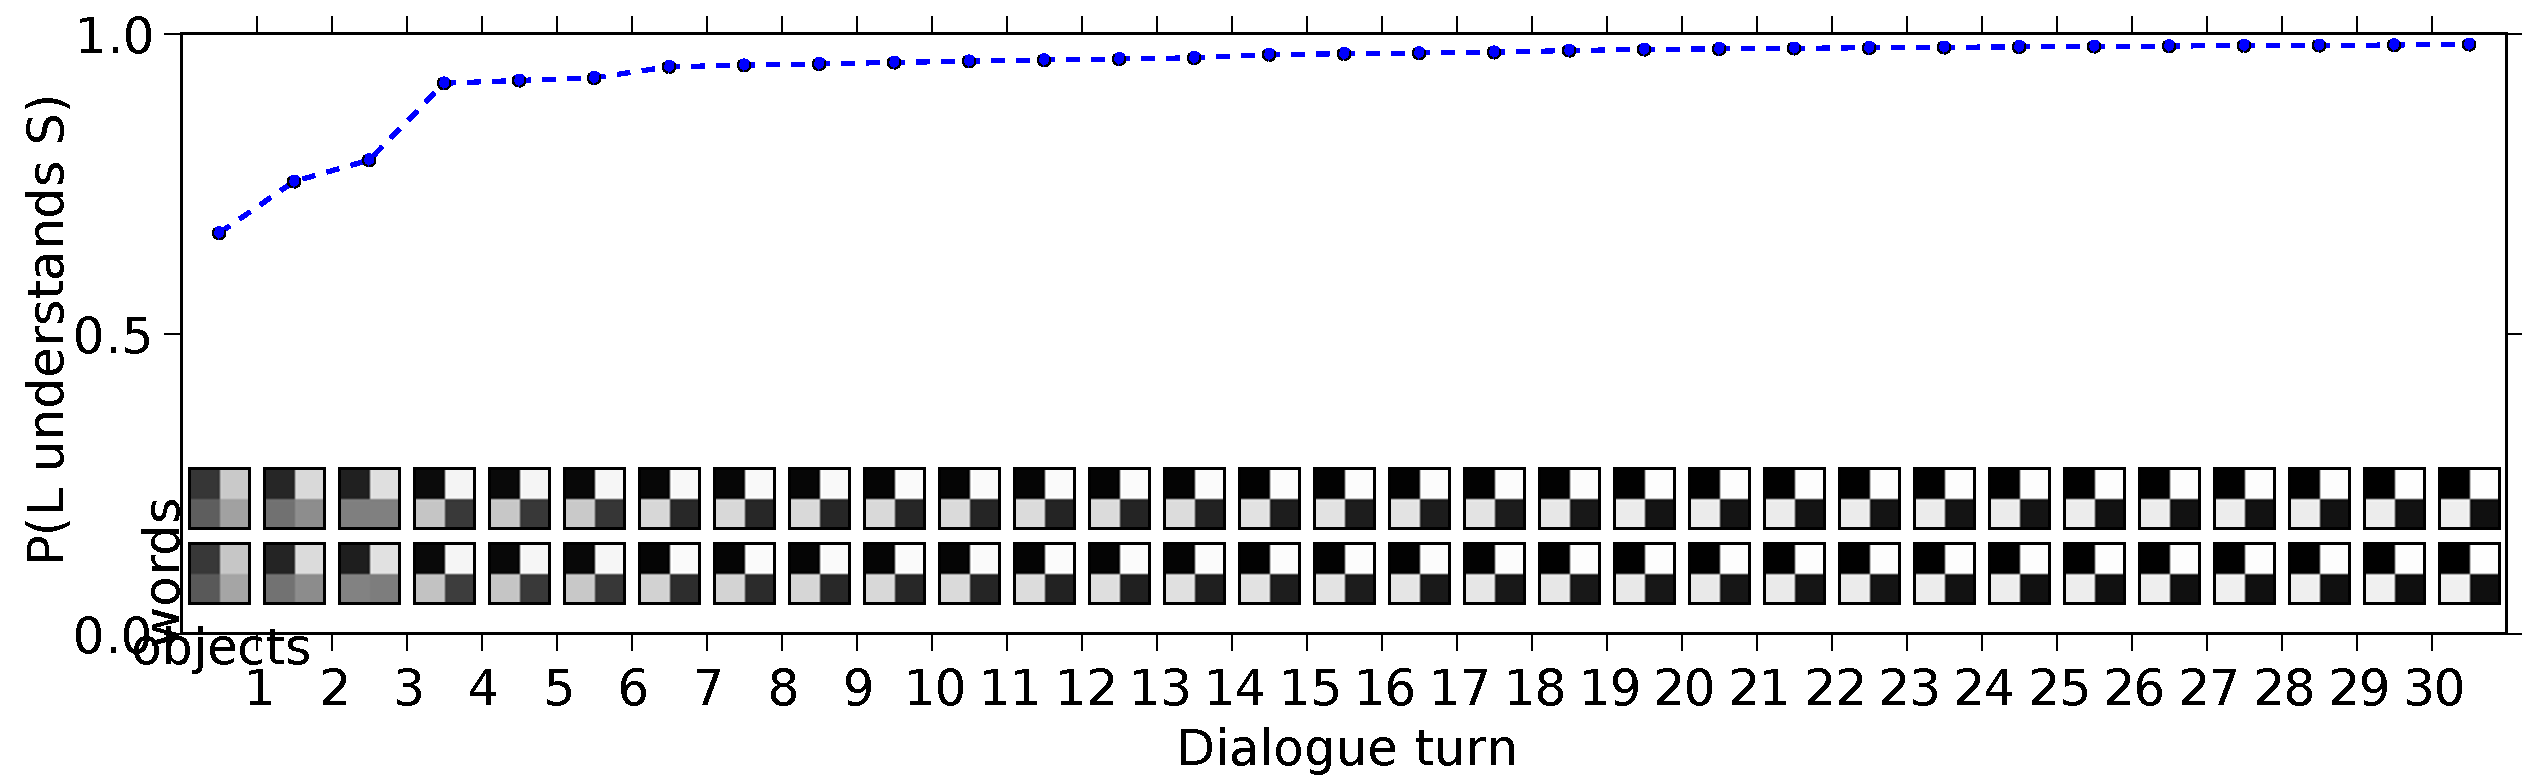
\includegraphics[width=0.48\textwidth]{figures/horn-emergence-0.pdf}
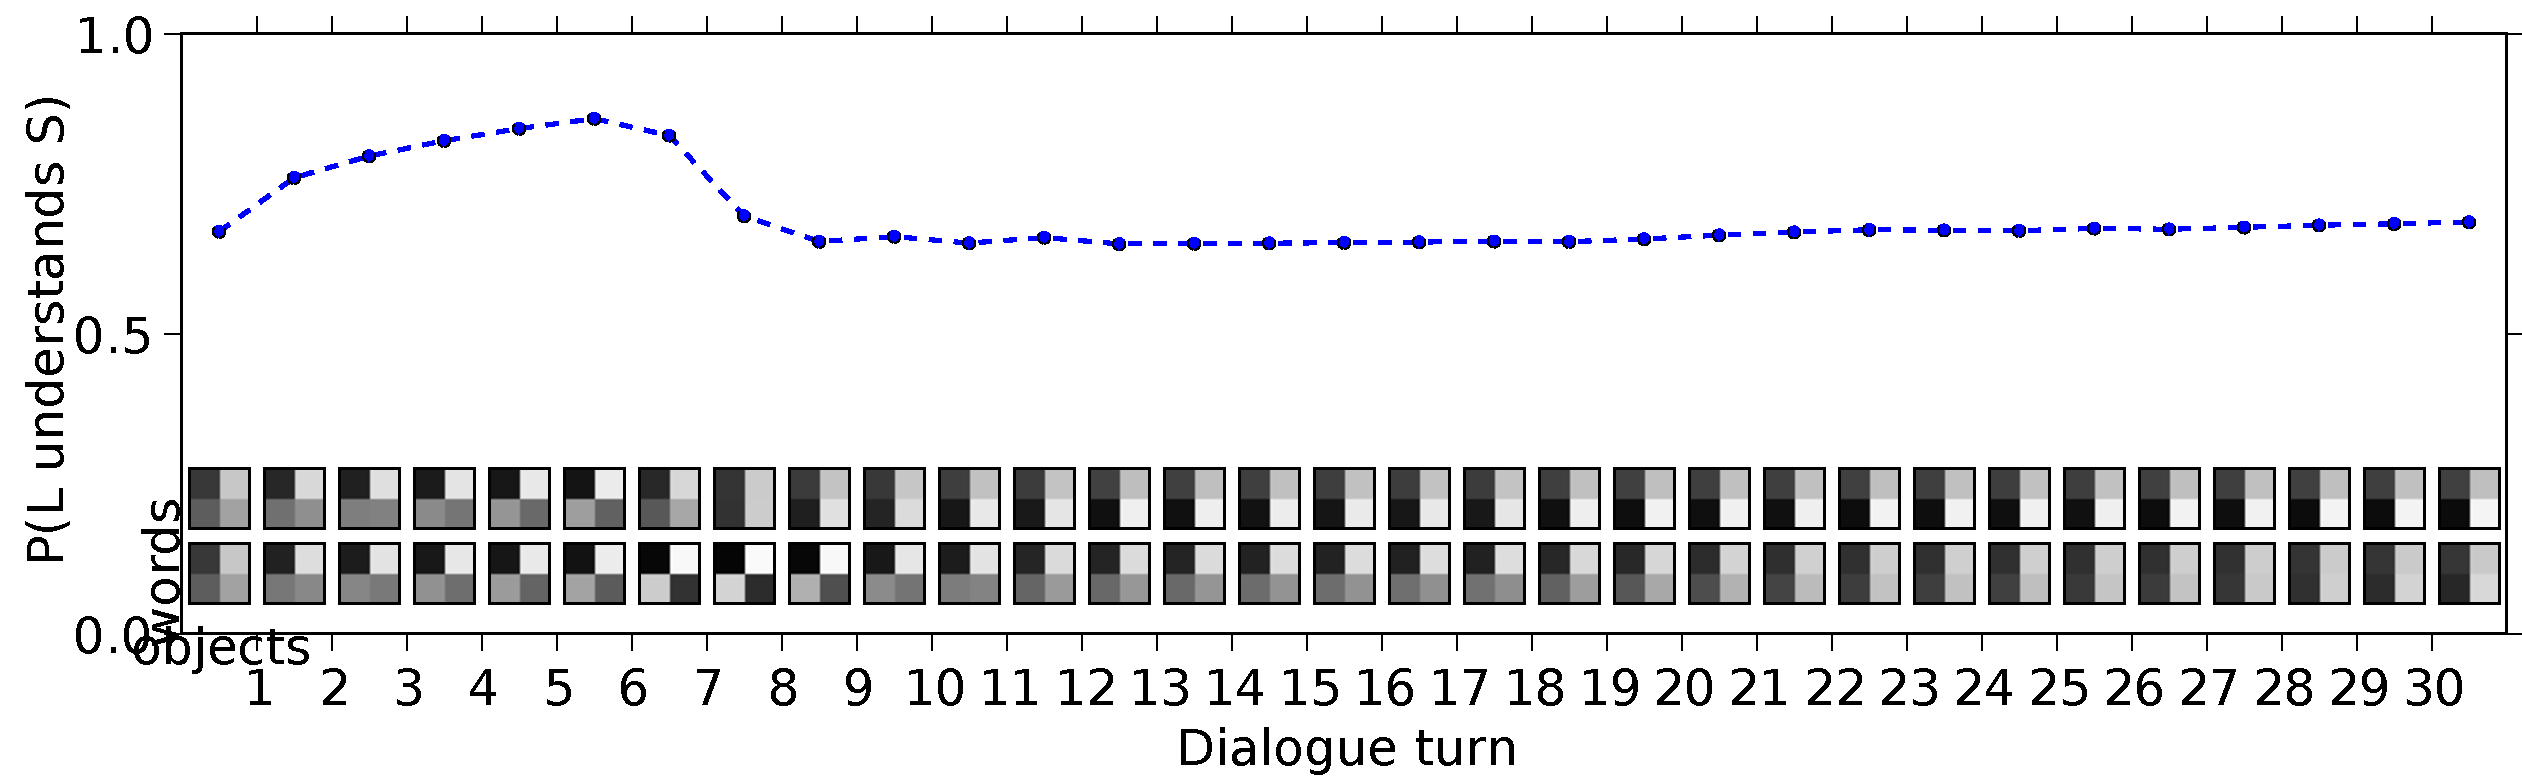
\includegraphics[width=0.48\textwidth]{figures/horn-emergence-1.pdf}
\caption{\label{fig:horn} Simulations.}
\end{figure}

% To show that they're lexicalized, at end of each of 4 dialogues, we
% look at how speaker and listener talk about/interpret the objects/words:
%
% Dialogue 0, after disabling implicature:
%   How speaker refers to "common" and "rare" objects:
% array([[  9.99994601e-01,   1.67862018e-02],
%        [  5.39888463e-06,   9.83213798e-01]])
%   Listener's interpretation of "cheap" and "expensive" words:
% array([[ 0.84765063,  0.15234937],
%        [ 0.02451694,  0.97548306]])

% Dialogue 1, after disabling implicature:
%   How speaker refers to "common" and "rare" objects:
% array([[  9.99997339e-01,   1.04639034e-02],
%        [  2.66058112e-06,   9.89536097e-01]])
%   Listener's interpretation of "cheap" and "expensive" words:
% array([[ 0.86951534,  0.13048466],
%        [ 0.01986478,  0.98013522]])

% Dialogue 2, after disabling implicature:
%   How speaker refers to "common" and "rare" objects:
% array([[  9.99984637e-01,   2.19135388e-02],
%        [  1.53629560e-05,   9.78086461e-01]])
%   Listener's interpretation of "cheap" and "expensive" words:
% array([[ 0.83486332,  0.16513668],
%        [ 0.03421814,  0.96578186]])

% Dialogue 3, after disabling implicature:
%   How speaker refers to "common" and "rare" objects:
% array([[  9.99996148e-01,   1.92821280e-02],
%        [  3.85172462e-06,   9.80717872e-01]])
%   Listener's interpretation of "cheap" and "expensive" words:
% array([[ 0.83985034,  0.16014966],
%        [ 0.02170542,  0.97829458]])


\subsection{Lexicalization and preservation of scalar implicature}


\begin{figure}
\centering
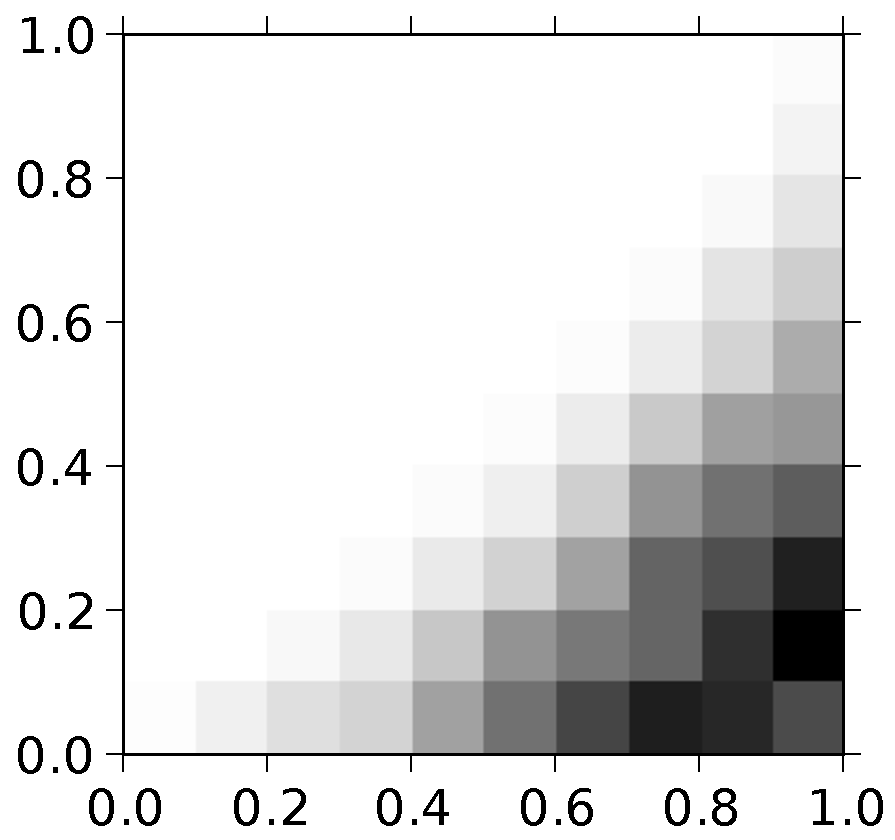
\includegraphics[width=2in]{figures/some-all-only-pragmatic.pdf}
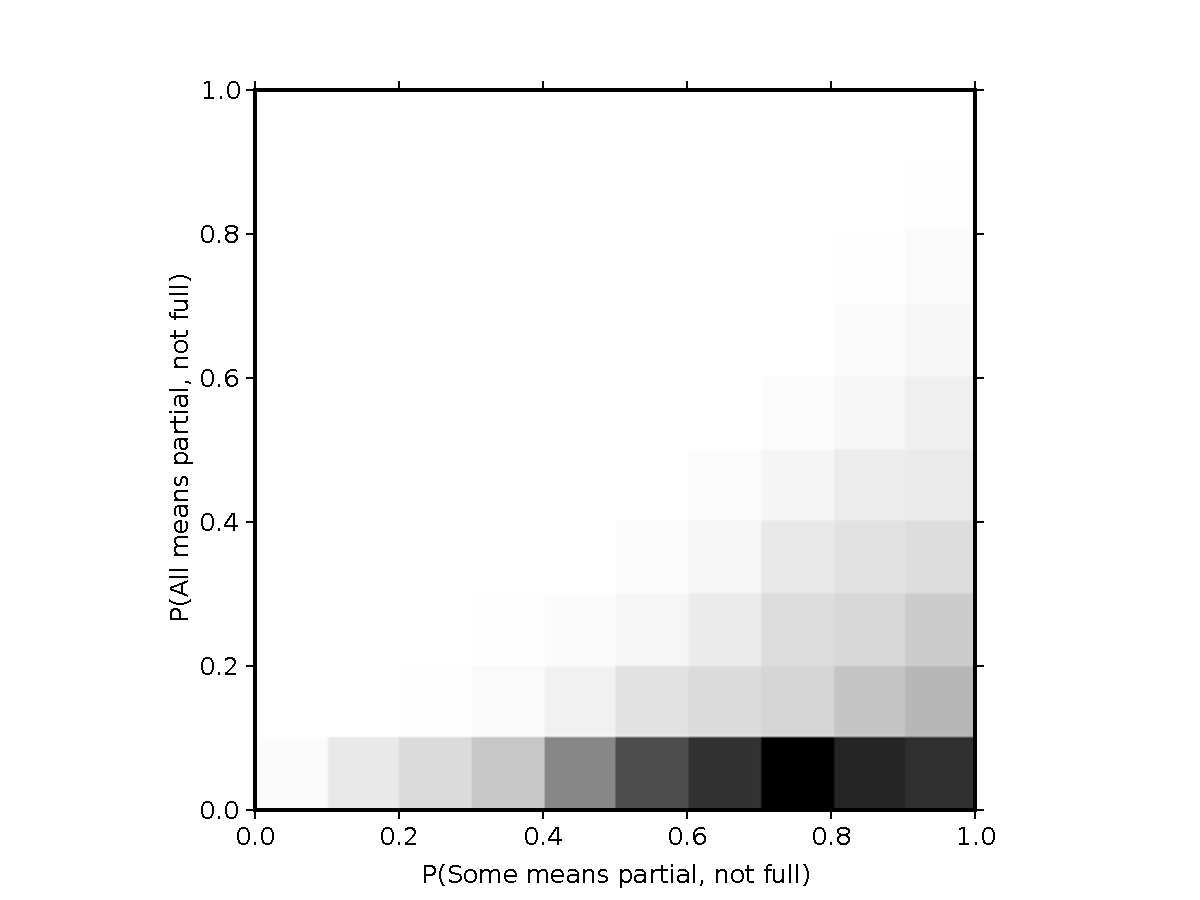
\includegraphics[width=2in]{figures/some-all-pragmatic+unambiguous.pdf}
\caption{\label{fig:scalar} Simulations..}
\end{figure}

\section{Conclusion}

%\subsubsection*{Acknowledgments}


% Thanks to ONR Grant #blahblah


\bibliographystyle{plain}
\bibliography{pragmatics}

\end{document}
